% fig3_equiv_dist — energy-equivalent distance transform (创新点1)
% 用途: 交底书 图3, §五 S1 定义 EED(i,j,L)=d_ij*(alpha+beta L)/alpha
% 要点: 同一几何边因出发载重不同 EED 不同 -> 顺序影响总 EED
% 公式: A3_REQUIREMENTS.md §3.2 / energy_model.py compute_equiv_distance
% 编译: latexmk -pdf -xelatex fig3_equiv_dist.tex
\documentclass[tikz,border=8pt]{standalone}
\usepackage{amsmath}
\usepackage{tikz}
\usetikzlibrary{arrows.meta}
\begin{document}
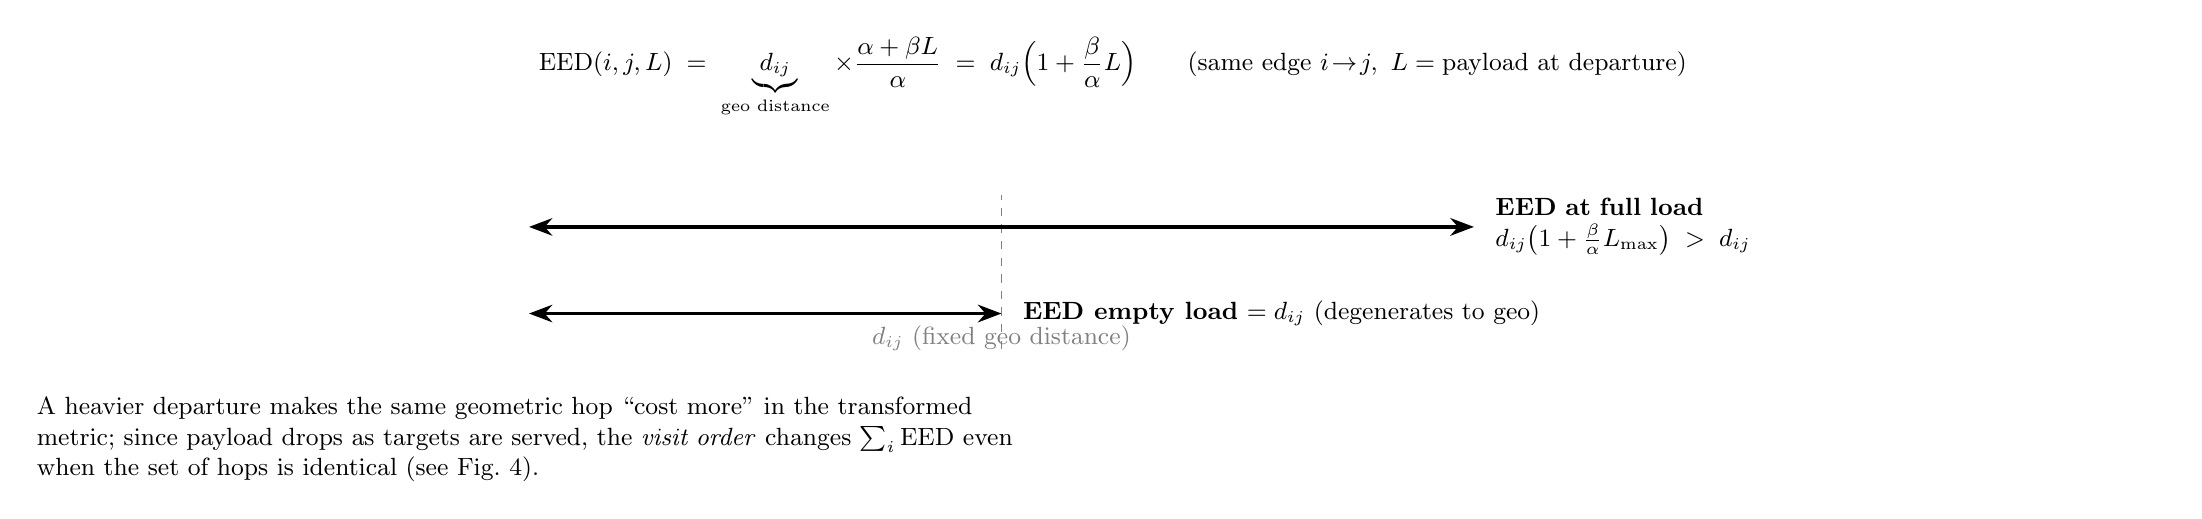
\begin{tikzpicture}[font=\small]
% --- top: definition ---
\node[anchor=west] (f) at (0,3.6) {
  $\mathrm{EED}(i,j,L)\;=\;\underbrace{d_{ij}}_{\text{geo distance}}
   \times\dfrac{\alpha+\beta L}{\alpha}\;=\;
   d_{ij}\Bigl(1+\dfrac{\beta}{\alpha}L\Bigr)
   \qquad\text{(same edge } i\!\to\!j,\ L=\text{payload at departure)}$};

% --- vertical guide at x=6 marking the geometric distance ---
\draw[dashed, gray] (6,0.15) -- (6,2.1);
\node[gray,anchor=south] at (6,0.0) {$d_{ij}$ (fixed geo distance)};

% --- EED full load (longer) ---
\draw[very thick, {Stealth}-{Stealth[length=3mm]}] (0,1.7) -- (12,1.7);
\node[anchor=west,text width=8.5cm,align=left] at (12.15,1.7) {\textbf{EED at full load}\\
  $d_{ij}\bigl(1+\tfrac{\beta}{\alpha}L_{\max}\bigr) \;>\; d_{ij}$};

% --- EED empty (equals geo) ---
\draw[very thick, {Stealth}-{Stealth[length=3mm]}] (0,0.6) -- (6,0.6);
\node[anchor=west] at (6.15,0.6) {\textbf{EED empty load} $= d_{ij}$\ (degenerates to geo)};

% --- caption ---
\node[text width=12.5cm,align=left,font=\small] at (0,-1.0) {
  A heavier departure makes the same geometric hop ``cost more'' in the transformed metric;
  since payload drops as targets are served, the \emph{visit order} changes $\sum_i\mathrm{EED}$ even
  when the set of hops is identical (see Fig.~4).};
\end{tikzpicture}
\end{document}
